\documentclass{beamer}
\usetheme{Madrid}
\usepackage{graphicx}
\usepackage{array}
\usepackage{ragged2e}
\usepackage{comment}
\usepackage{amsmath}
\usepackage{tikz}
\usepackage{pgfplots}
\pgfplotsset{compat=1.18}
\usepackage{booktabs}
\usepackage{algorithm}
\usepackage{algpseudocode}
\usepackage{longtable}
\usetikzlibrary{patterns, shapes.geometric, arrows, positioning}

\setbeamertemplate{footline}{}
\setbeamertemplate{navigation symbols}{}

\title{AIInvigilator -- Real-Time Malpractice Detection in Classrooms Using Computer Vision}
\author{
  Abhishek R S \quad MDL22CSBS004\\
  Faris Abdul Raoof Arakkal \quad MDL22CSBS020\\
  R Pranav \quad MDL22CSBS049\\
  Sarang Santhosh Kumar \quad MDL22CSBS051
}
\date{\today}

\begin{document}

% ================================================================
%  TITLE
% ================================================================
\begin{frame}
    \titlepage
\end{frame}

% ================================================================
%  TABLE OF CONTENTS
% ================================================================
\begin{frame}{Contents}
  \tableofcontents[sections={1-8}]
\end{frame}

\begin{frame}{Contents (contd.)}
  \tableofcontents[sections={9-16}]
\end{frame}

% ================================================================
\section{Introduction}
% ================================================================
\begin{frame}{Introduction}
\begin{itemize}
    \item Traditional human invigilation is prone to fatigue, distractions, and oversight in crowded or long-duration exams.
    \item Existing CCTV monitoring lacks real-time intelligence and requires manual review.
    \item Rising instances of subtle cheating highlight the need for \textbf{automated, intelligent monitoring}.
    \item \textbf{AIInvigilator} integrates advanced computer vision techniques to fill this gap.
    \item Provides a \textbf{scalable, resource-efficient solution optimized for mid-tier GPU-enabled classroom environments}, assisting invigilators and improving exam fairness.
\end{itemize}
\end{frame}

% ================================================================
\section{Abstract}
% ================================================================
\begin{frame}{Abstract}
\begin{itemize}
    \item \textbf{AIInvigilator} is a real-time AI-powered system developed to detect examination malpractices in classrooms.
    \item Employs \textbf{YOLO for object detection} and \textbf{pose estimation} to recognize cheating behaviors.
    \item Identifies suspicious activities such as mobile phone use, note exchanges, and abnormal gestures.
    \item Generates \textbf{real-time alerts} and maintains logs with \textbf{time-stamped evidence} for review.
    \item Optimized for \textbf{moderate computational resources}, making it scalable and practical.
    \item Aims to enhance academic integrity with a \textbf{fair, efficient, and automated} monitoring solution.
\end{itemize}
\end{frame}

% ================================================================
\section{Problem Statement}
% ================================================================
\begin{frame}{Problem Statement}
Existing exam proctoring solutions are often fragmented, overly theoretical, or impractical for large-scale deployment. Many models are validated only on limited, lab-specific datasets and fail to generalize to real-world exam conditions. Current approaches focus on a narrow range of behaviors and lack an integrated multi-modal framework. Absence of complete end-to-end systems combining real-time detection, dashboards, logging, and feedback loops. Hence, a robust, scalable, and real-world deployable system is required.
\end{frame}

% ================================================================
\section{Objectives}
% ================================================================
\begin{frame}{Objectives}
\begin{itemize}
  \item Detect students, mobile phones, and notes in real time using object detection.
  \item Recognize suspicious gestures (e.g., turning back, leaning) via pose estimation.
  \item Send real-time alerts to invigilators when malpractice is detected.
  \item Log incidents with time-stamped visual evidence for post-exam analysis.
  \item Enable deployment on low-end devices through model optimization.
\end{itemize}
\end{frame}

% ================================================================
\section{Our Solution: AIInvigilator}
% ================================================================
\begin{frame}{Our Solution: AIInvigilator}
\begin{itemize}
  \item Comprehensive, end-to-end system addressing gaps in academic integrity solutions.
  \item Leverages YOLO for object detection and pose estimation.
  \item Trained on a diverse custom dataset for better generalization.
  \item Provides workflow: real-time alerts, video evidence, dashboard, and robust logging.
  \item Optimized for low-resource hardware, operating on secure LAN for scalability and privacy.
\end{itemize}
\end{frame}

% ================================================================
\section{Literature Survey}
% ================================================================
\begin{frame}{}
    \centering
    \Huge Literature Survey
\end{frame}

\begin{frame}{Literature Survey -- Papers 1--5}
\centering
\resizebox{\textwidth}{!}{%
\begin{tabular}{|p{3cm}|p{2.5cm}|p{3.5cm}|p{3cm}|p{3.5cm}|}
\hline
\textbf{Title} & \textbf{Authors} & \textbf{Key Findings} & \textbf{Advantages} & \textbf{Disadvantages} \\
\hline
AI-based Surveillance for Exam Integrity &
Adhatrao et al. &
YOLOv8 real-time monitoring; 85.34\% precision, 12.94 ms/frame &
High speed, real-time alerts &
Lower recall (65\%) \\
\hline
Students' Perceptions Toward Cheating in Online Education &
Rodriguez et al. &
Survey: e-auth awareness prevents cheating &
User-centric context, psychological deterrent &
Technology alone insufficient \\
\hline
Cheating Detection Using Improved YOLOv8 &
Zuo et al. &
ECA attention; 82.71\% acc, 27 FPS &
Real-time, outperforms SSD &
Needs manual confirmation \\
\hline
YOLOv8n\_BT Behavior Recognition &
Liu et al. &
BRA + TODL; +6.7\% Recall, 312 FPS &
High speed, strong generalization &
Single school dataset \\
\hline
What Is YOLOv8: An In-Depth Exploration &
Yaseen et al. &
Anchor-free, CSPNet backbone, enhanced augmentation &
Higher mAP, faster inference &
Review paper only \\
\hline
\end{tabular}%
}
\end{frame}

\begin{frame}{Literature Survey -- Papers 6--10}
\centering
\resizebox{\textwidth}{!}{%
\begin{tabular}{|p{3cm}|p{2.5cm}|p{3.5cm}|p{3cm}|p{3.5cm}|}
\hline
\textbf{Title} & \textbf{Authors} & \textbf{Key Findings} & \textbf{Advantages} & \textbf{Disadvantages} \\
\hline
Cheating Recognition (SE-YOLOv8) &
Lu et al. &
SE-YOLOv8 + 3D CNN; 91.6\% acc, 96\% mAP50 &
Multi-stage, high accuracy &
Non-public dataset \\
\hline
Anomaly Detection for Online Examination &
Ebron et al. &
YOLOv8 + MediaPipe; 97.9\% mAP for phones &
Standard hardware, high accuracy &
Lab environment only \\
\hline
Cross-Domain Multitask Model for Head Detection &
Bafti et al. &
Mask-RCNN + ResNet-50; 6--8° MAE pose &
Integrated pipeline, cross-domain &
Not real-time ($\sim$16 FPS) \\
\hline
Real-Time Student Engagement Monitoring &
Albohamood et al. &
YOLO + Pose; F1=0.96, Precision=1.00 &
Very high performance, web dashboard &
Small dataset ($\sim$2000 images) \\
\hline
Video Processing Using Deep Learning &
Sharma et al. &
Reviewed 93 studies: CNN, RNN, hybrid models &
Broad overview, key trends &
Review ends 2020, misses YOLOv8 \\
\hline
\end{tabular}%
}
\end{frame}

\begin{frame}{Literature Survey -- Papers 11--15}
\centering
\resizebox{\textwidth}{!}{%
\begin{tabular}{|p{3cm}|p{2.5cm}|p{3.5cm}|p{3cm}|p{3.5cm}|}
\hline
\textbf{Title} & \textbf{Authors} & \textbf{Key Findings} & \textbf{Advantages} & \textbf{Disadvantages} \\
\hline
Exam Guard: Enhanced Academic Integrity &
Gisto et al. &
YOLOv5 + MediaPipe; mAP@50=0.987 for phones &
High task accuracy, web dashboard &
Lower on complex gestures (0.716) \\
\hline
Classification of Violations in Exam Rooms &
Shen et al. &
DenseNet 95.62\% accuracy on 95K images &
High classification accuracy &
No localization, image-class only \\
\hline
TeacherEye: AI-Powered Engagement Monitoring &
Abdelhadi et al. &
DeepFace + Whisper + VLM multimodal &
Multi-modal, VLM intervention &
Complex, external APIs, privacy risk \\
\hline
Automatic Object Detection for Behavioral Research &
Hermens et al. &
YOLOv8 near-perfect on small datasets (100--350 img) &
Easy to use, small dataset effective &
Poor cross-environment generalization \\
\hline
Improved YOLOv8 to Detect Moving Objects &
Safaldini et al. &
Ghost blocks + Wise-IoU loss; 90\% acc, 30 FPS &
Edge device support (Jetson Nano) &
Complex to replicate, vehicle-focused \\
\hline
\end{tabular}%
}
\end{frame}

\begin{frame}{Literature Survey -- Inferences for AIInvigilator}
\centering
\resizebox{\textwidth}{!}{%
\begin{tabular}{|p{3.5cm}|p{8cm}|}
\hline
\textbf{Paper} & \textbf{Inference for AIInvigilator} \\
\hline
Adhatrao et al. & Confirms YOLOv8 is viable for real-time invigilation \\
\hline
Rodriguez et al. & Justifies proctoring as a behavioral deterrent \\
\hline
Zuo et al. & Attention mechanisms improve subtle cheating detection \\
\hline
Liu et al. & Architectural improvements for crowded classrooms \\
\hline
Yaseen et al. & Strong justification for YOLOv8 as core model \\
\hline
Lu et al. & Hierarchical keyframe approach for efficiency \\
\hline
Ebron et al. & Validates YOLO + pose tool combination \\
\hline
Bafti et al. & Suggests future multitask learning path \\
\hline
Albohamood et al. & Confirms YOLO + pose for student behavior classification \\
\hline
Sharma et al. & Validates CNN + temporal logic as state-of-the-art \\
\hline
Gisto et al. & Strong validation of YOLO + pose approach \\
\hline
Shen et al. & Suggests DenseNet classifier + YOLO hybrid approach \\
\hline
Abdelhadi et al. & Ideas for future audio analysis and VLM integration \\
\hline
Hermens et al. & Diverse training data required for classroom scaling \\
\hline
Safaldini et al. & Wise-IoU loss for detecting subtle student movements \\
\hline
\end{tabular}%
}
\end{frame}

% ================================================================
\section{Key Innovations}
% ================================================================
\begin{frame}{Key Innovations}
\begin{itemize}
    \item \textbf{Hybrid Detection Architecture:} Combines YOLOv11n object detection with YOLO-Pose (YOLOv8n-pose) keypoint analysis and rule-based CV logic.
    \item \textbf{Real-Time WebSocket Streaming:} Frame-level ML processing using Django Channels and Redis for low-latency live monitoring.
    \item \textbf{Consecutive Frame Thresholding:} Eliminates momentary false positives by requiring persistent detection (3--5 frames).
    \item \textbf{Grace Period Mechanism:} Continues recording for 60 frames ($\approx 2$ seconds) post-detection to capture complete incident context.
\end{itemize}
\end{frame}

\begin{frame}{AI Probability Scoring Engine}
Computes a confidence score (0--100) for each event to reduce false positives. Uses five weighted factors:
\begin{itemize}
    \item \textbf{Clip Duration (30\%):} Longer clips yield higher confidence.
    \item \textbf{Detection Frame Density (25\%):} Higher detection frequency increases confidence.
    \item \textbf{Malpractice Type Prior (20\%):} Type-specific false positive rates (e.g., Mobile: 0.80).
    \item \textbf{Detection Sustainability (15\%):} How far above threshold the detection persists.
    \item \textbf{Base Confidence (10\%):} Baseline from the ML model.
\end{itemize}
\end{frame}

% ================================================================
%  PROJECT DESIGN DIVIDER
% ================================================================
\begin{frame}{}
    \centering
    \Huge Project Design
\end{frame}

% ================================================================
\section{System Diagrams}
% ================================================================
\subsection{Overall System Architecture}
\begin{frame}{Overall System Architecture}
    \begin{figure}
        \centering
        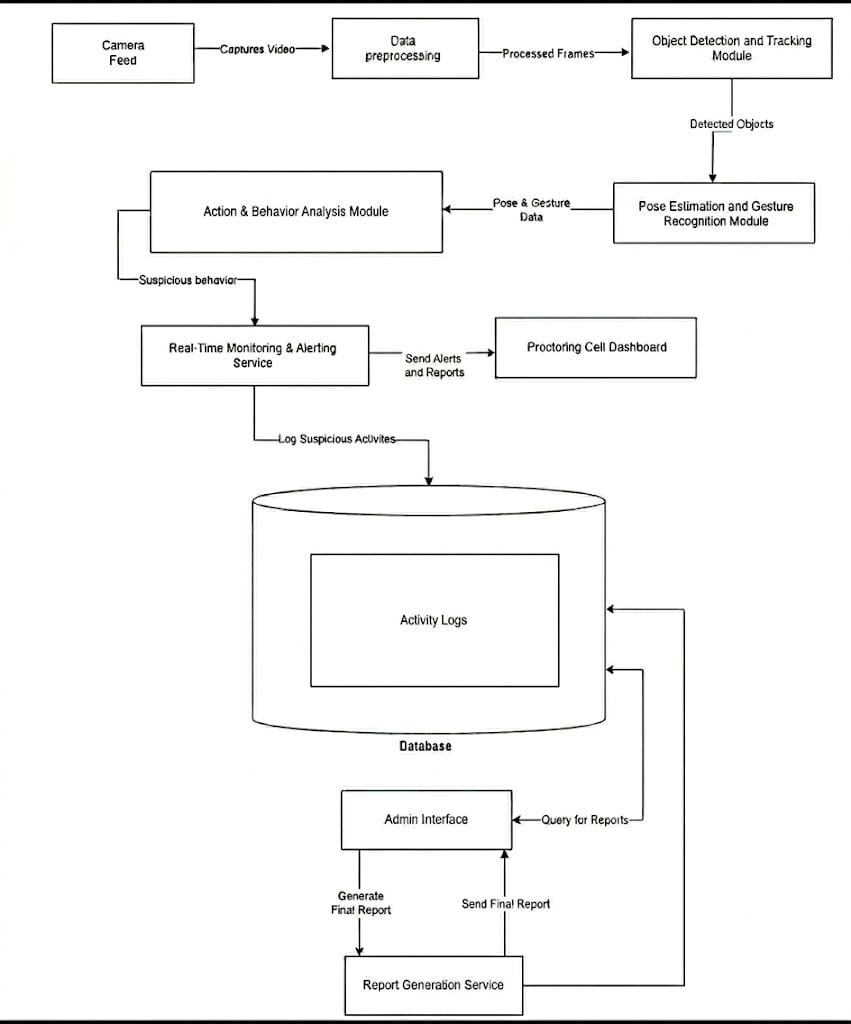
\includegraphics[height=0.8\textheight, keepaspectratio]{architecture.jpeg}
        \caption{Overall flow from video capture through analysis to alerts and storage.}
    \end{figure}
\end{frame}

\subsection{DFD Level 0}
\begin{frame}{DFD Level 0}
    \begin{figure}
        \centering
        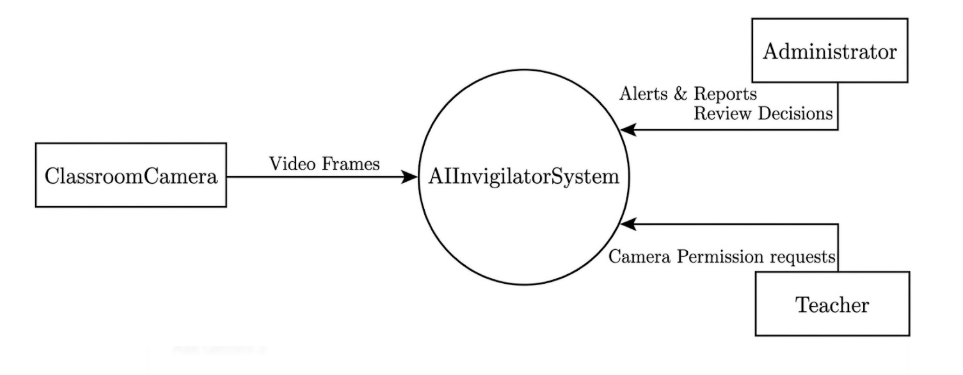
\includegraphics[width=\textwidth, keepaspectratio]{dfd0.jpeg}
        \caption{Data Flow Diagram Level 0 showing the overall system.}
    \end{figure}
\end{frame}

\subsection{DFD Level 1}
\begin{frame}{DFD Level 1}
    \begin{figure}
        \centering
        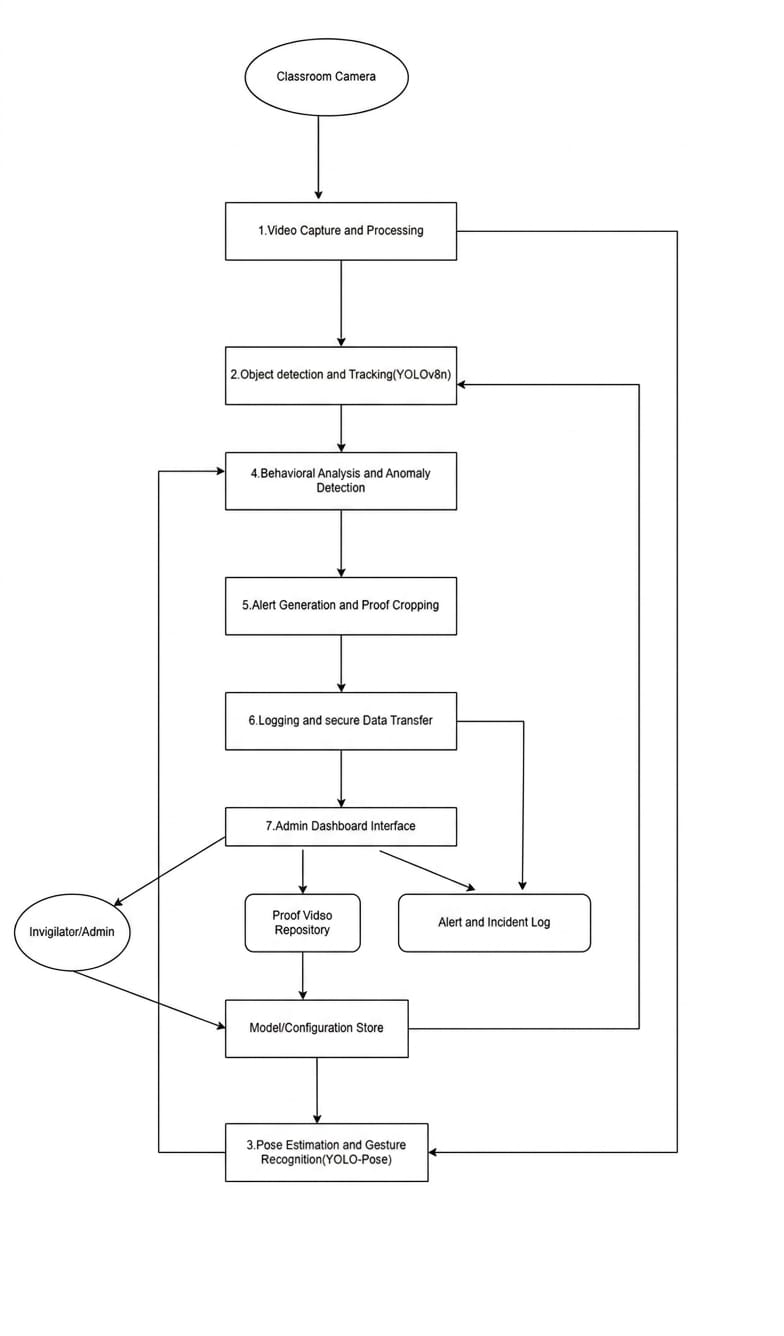
\includegraphics[height=0.8\textheight, keepaspectratio]{dfd1.jpeg}
        \caption{Data Flow Diagram Level 1 showing detailed internal processes.}
    \end{figure}
\end{frame}

\subsection{FlowChart Diagram}
\begin{frame}{FlowChart Diagram}
    \begin{figure}
        \centering
        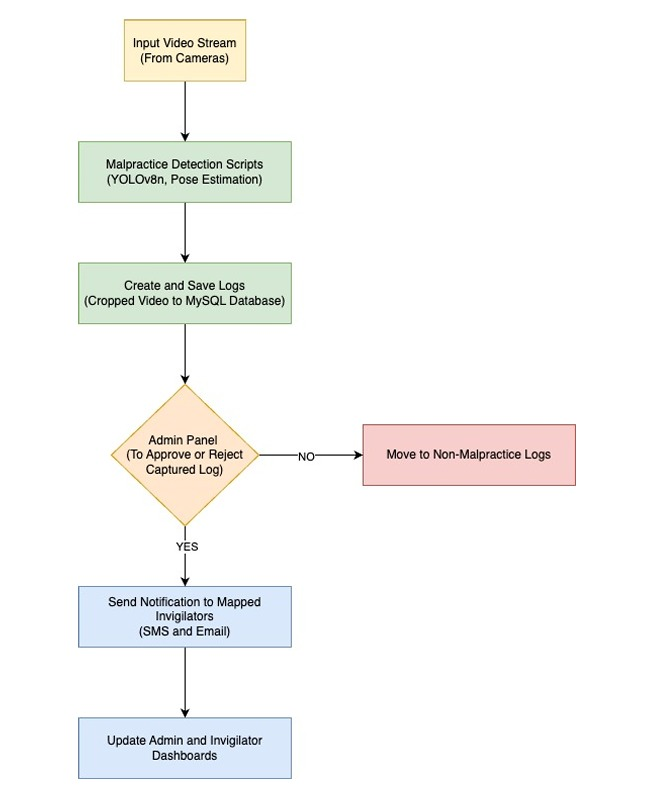
\includegraphics[height=0.8\textheight, keepaspectratio]{block_diagram.jpg}
        \caption{A diagram illustrating the system's sequential workflow.}
    \end{figure}
\end{frame}

\subsection{Use Case Diagram}
\begin{frame}{Use Case Diagram}
    \begin{figure}
        \centering
        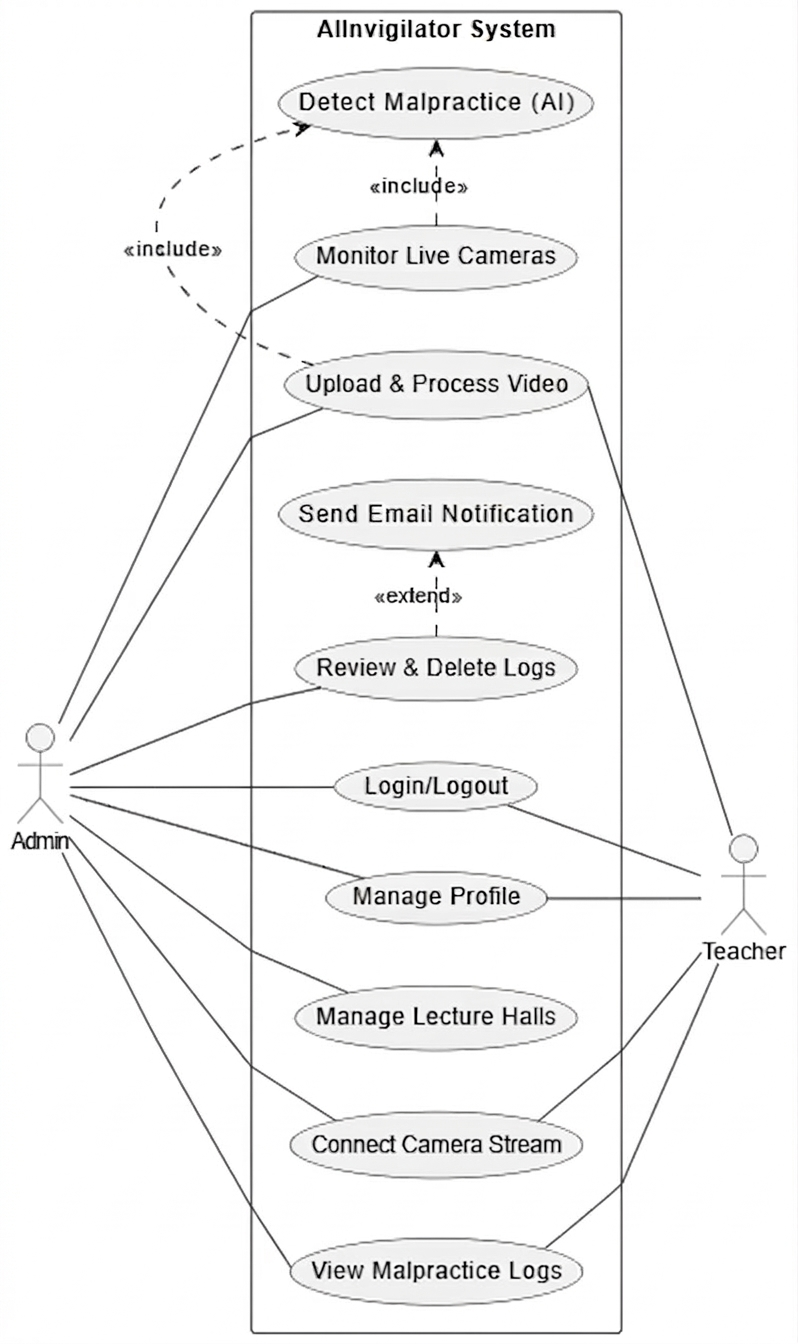
\includegraphics[height=0.8\textheight, keepaspectratio]{usecase.png}
        \caption{Use Case Diagram representing interactions between users and the system.}
    \end{figure}
\end{frame}

% ================================================================
\section{System Architecture}
% ================================================================
\begin{frame}{System Architecture}
    \begin{itemize}
        \item The AIInvigilator system employs a \textbf{modular, real-time, and offline-first} architectural design.
        \item This approach ensures data privacy, low latency, and robust operation without requiring an internet connection.
        \item The architecture consists of several interconnected components responsible for video processing, AI-based analysis, and data management.
        \item It is designed to run on local hardware, with secure and anonymized data transfer to a central server for review.
    \end{itemize}
\end{frame}

% ================================================================
\section{Modules and Module Descriptions}
% ================================================================
\begin{frame}{Modules Overview}
    Our system is broken down into several key modules, each with a specific function:
    \begin{enumerate}
        \item Camera Feed Module
        \item Data Preprocessing Module
        \item Object Detection Module (YOLO)
        \item Pose Estimation \& Gesture Recognition
        \item Action Recognition and Behaviour Analysis Module
        \item Real-Time Monitoring \& Alerting
        \item Proctoring Cell Dashboard
        \item Database Logging System
    \end{enumerate}
\end{frame}

\begin{frame}{Camera Feed Module}
\begin{itemize}
    \item Captures live video using OpenCV
    \item Supports webcam and video file input
    \item Provides continuous frame stream to detection pipeline
    \item Works in real-time during examination
\end{itemize}
\end{frame}

\begin{frame}{Data Preprocessing}
\begin{itemize}
    \item Downscaling of frame quality for optimized inference
    \item FPS control for real-time performance
    \item Frame-by-frame processing pipeline
    \item Prepares frames for YOLO model input
\end{itemize}
\end{frame}

\begin{frame}{Object Detection Module}
\begin{itemize}
    \item Uses YOLO model for detection
    \item Detects students and suspicious objects
    \item Mobile phone detection supported
    \item Runs in real-time
\end{itemize}
\end{frame}

\begin{frame}{Pose Estimation \& Gesture Recognition}
\begin{itemize}
    \item Uses YOLO Pose model
    \item Extracts body keypoints
    \item Detects posture changes
\end{itemize}
\end{frame}

\begin{frame}{Action Recognition and Behaviour Analysis Module}
\begin{itemize}
    \item Detects:
    \begin{itemize}
        \item Leaning
        \item Turning Back
        \item Hand Raising
        \item Passing Objects
    \end{itemize}
    \item Based on pose and object detection outputs
    \item Applies rule-based thresholds
    \item Identifies suspicious activities
\end{itemize}
\end{frame}

% ================================================================
\section{Rule-Based CV Analysis}
% ================================================================
\begin{frame}{Rule-Based CV Analysis Details}
Analyzes pose keypoints to classify specific malpractice behaviors:
\begin{itemize}
    \item \textbf{Mobile Phone:} Identifies COCO class 67 objects with a 5-frame consecutive threshold.
    \item \textbf{Leaning:} Computes horizontal head shift from the shoulder center midpoint.
    \item \textbf{Turning Back:} Analyzes head angle deviation by comparing ear-to-nose distance ratios.
    \item \textbf{Passing Paper:} Detects hand-to-hand proximity between adjacent students.
    \item \textbf{Hand Raised:} Checks if wrist keypoints are significantly above the corresponding shoulder threshold.
\end{itemize}
\end{frame}

% ================================================================
%  ALGORITHMS DIVIDER
% ================================================================
\begin{frame}{}
    \centering
    \Huge Algorithms
\end{frame}

% ================================================================
\section{Algorithms}
% ================================================================

\begin{frame}{Algorithm 1 -- Frame Processing Pipeline}
\begin{columns}
\begin{column}{0.5\textwidth}
\footnotesize
\textbf{Description:}\\
Core pipeline that receives a WebSocket frame, runs YOLOv8n + YOLO-Pose, applies rule-based CV analysis, manages consecutive counters, and returns an annotated frame.\\[0.3cm]
\textbf{Steps:}
\begin{enumerate}\footnotesize
    \item Accept JPEG-encoded frame
    \item Decode \& preprocess (resize)
    \item Run YOLOv8n object detection
    \item Run YOLO-Pose estimation
    \item Apply CV rules per person
    \item Threshold check per type
    \item Return annotated frame
\end{enumerate}
\end{column}
\begin{column}{0.5\textwidth}
\begin{algorithmic}[1]
\footnotesize
\Function{ProcessFrame}{$frameBytes, streamId$}
  \State $frame \gets$ DecodeJPEG($frameBytes$)
  \State $frame \gets$ Resize($frame$)
  \State $objects \gets$ YOLOv8n.detect($frame$)
  \State $poses \gets$ YOLOPose.estimate($frame$)
  \State $detections \gets []$
  \For{each $person$ in $poses$}
    \State $kp \gets person$.keypoints
    \If{DetectMobile($objects, kp$)}
      \State IncrCounter($streamId$, ``mobile'')
    \EndIf
    \If{DetectLeaning($kp$)}
      \State IncrCounter($streamId$, ``lean'')
    \EndIf
    \For{each $type$}
      \If{Counter $\geq$ Threshold($type$)}
        \State Append $type$ to $detections$
      \EndIf
    \EndFor
  \EndFor
  \State \Return Annotate($frame, detections$)
\EndFunction
\end{algorithmic}
\end{column}
\end{columns}
\end{frame}

\begin{frame}{Algorithm 2 -- Mobile Phone Detection}
\begin{columns}
\begin{column}{0.48\textwidth}
\footnotesize
\textbf{Description:}\\
Detects COCO class 67 (``cell phone'') in YOLOv8n output. Requires detection in \textbf{5 consecutive frames} before flagging, with a 60-frame grace period.\\[0.3cm]
\textbf{Key Parameters:}
\begin{itemize}\footnotesize
    \item Confidence threshold: $\tau = 0.25$
    \item Must be near a wrist keypoint
    \item Oversized bbox rejected if area $> 15\%$ of frame
    \item Near-square aspect ratio rejected
    \item Consecutive threshold: 5 frames
\end{itemize}
\end{column}
\begin{column}{0.52\textwidth}
\begin{algorithmic}[1]
\footnotesize
\Function{DetectMobile}{$objects, keypoints$}
  \For{each $obj$ in $objects$}
    \If{$obj$.class $= 67$}
      \If{$obj$.conf $\geq 0.25$}
        \If{IsNearHand($obj$.bbox, $keypoints$.wrists)}
          \State \Return \textbf{True}
        \EndIf
      \EndIf
    \EndIf
  \EndFor
  \State \Return \textbf{False}
\EndFunction
\end{algorithmic}
\vspace{0.4cm}
\begin{block}{\footnotesize Smart Filters}
\footnotesize Rejects oversized bboxes and near-square aspect ratios at low confidence to avoid false positives from calculators and desk objects.
\end{block}
\end{column}
\end{columns}
\end{frame}

\begin{frame}{Algorithm 3 -- Leaning Detection}
\begin{columns}
\begin{column}{0.48\textwidth}
\footnotesize
\textbf{Description:}\\
Detects lateral leaning by computing the horizontal displacement of the nose from the shoulder midpoint, normalised by shoulder width.\\[0.3cm]
\textbf{Formula:}
\[
R_{\text{lean}} = \frac{|x_N - x_{SC}|}{W_S}
\]
\textbf{Key Parameters:}
\begin{itemize}\footnotesize
    \item $x_{SC}$: shoulder centre x-coordinate
    \item $W_S$: shoulder width
    \item Threshold: $R_{\text{lean}} > 0.4$
    \item Consecutive frames: 3
\end{itemize}
\end{column}
\begin{column}{0.52\textwidth}
\begin{algorithmic}[1]
\footnotesize
\Function{DetectLeaning}{$keypoints$}
  \State $SC \gets$ Midpoint($kp$.leftShoulder, $kp$.rightShoulder)
  \State $headShift \gets |kp$.nose.x $- SC$.x$|$
  \State $W_S \gets |kp$.leftShoulder.x $- kp$.rightShoulder.x$|$
  \If{$headShift > W_S \times 0.4$}
    \State \Return \textbf{True}
  \EndIf
  \State \Return \textbf{False}
\EndFunction
\end{algorithmic}
\vspace{0.4cm}
\begin{exampleblock}{\footnotesize Why Normalise?}
\footnotesize Dividing by $W_S$ makes the threshold resolution-independent --- the same rule works at 720p and 1080p.
\end{exampleblock}
\end{column}
\end{columns}
\end{frame}

\begin{frame}{Algorithm 4 -- Turning Back Detection}
\begin{columns}
\begin{column}{0.48\textwidth}
\footnotesize
\textbf{Description:}\\
Detects significant head rotation by analysing the ratio of nose-to-ear distances. When a student turns, one ear becomes occluded and the ratio drops.\\[0.3cm]
\textbf{Formula:}
\[
R_{\text{turn}} = \frac{\min(d_L, d_R)}{\max(d_L, d_R)}
\]
\textbf{Key Parameters:}
\begin{itemize}\footnotesize
    \item $d_L, d_R$: Euclidean nose-to-ear distances
    \item Threshold: $R_{\text{turn}} < 0.15$
    \item Captures rotation $> 60^\circ$
    \item Consecutive frames: 3
\end{itemize}
\end{column}
\begin{column}{0.52\textwidth}
\begin{algorithmic}[1]
\footnotesize
\Function{DetectTurning}{$keypoints$}
  \State $d_L \gets$ Dist($kp$.nose, $kp$.leftEar)
  \State $d_R \gets$ Dist($kp$.nose, $kp$.rightEar)
  \State $ratio \gets \dfrac{\min(d_L,d_R)}{\max(d_L,d_R)}$
  \If{$ratio < 0.15$}
    \State \Return \textbf{True}
  \EndIf
  \State \Return \textbf{False}
\EndFunction
\end{algorithmic}
\vspace{0.4cm}
\begin{block}{\footnotesize Geometric Intuition}
\footnotesize Face-forward: $R \approx 1.0$. At $60^\circ$: $R \approx 0.15$. Fully turned: $R \approx 0.0$.
\end{block}
\end{column}
\end{columns}
\end{frame}

\begin{frame}{Algorithm 5 -- Hand Raise Detection}
\begin{columns}
\begin{column}{0.48\textwidth}
\footnotesize
\textbf{Description:}\\
Detects raised hands by checking if either wrist keypoint is significantly above the shoulder keypoint in image coordinates ($y=0$ at top).\\[0.3cm]
\textbf{Formula:}
\[
\delta_W = y_{S,\min} - y_W
\]
\textbf{Key Parameters:}
\begin{itemize}\footnotesize
    \item $y_{S,\min}$: minimum shoulder y-value
    \item Threshold: $\delta_W > 20$ px
    \item \textbf{5 consecutive frames} (higher than others)
    \item Higher threshold because brief arm lifts are common
\end{itemize}
\end{column}
\begin{column}{0.52\textwidth}
\begin{algorithmic}[1]
\footnotesize
\Function{DetectHandRaised}{$keypoints$}
  \State $y_{S} \gets \min(kp$.leftShoulder.y, $kp$.rightShoulder.y$)$
  \If{$kp$.leftWrist.y $< y_S - 20$}
    \State \Return \textbf{True}
  \EndIf
  \If{$kp$.rightWrist.y $< y_S - 20$}
    \State \Return \textbf{True}
  \EndIf
  \State \Return \textbf{False}
\EndFunction
\end{algorithmic}
\vspace{0.4cm}
\begin{alertblock}{\footnotesize Note on Image Coords}
\footnotesize $y$ increases downward in image space, so wrist above shoulder means $y_W < y_S$, giving positive $\delta_W$.
\end{alertblock}
\end{column}
\end{columns}
\end{frame}

\begin{frame}{Algorithm 6 -- Passing Paper Detection}
\begin{columns}
\begin{column}{0.48\textwidth}
\footnotesize
\textbf{Description:}\\
Detects paper exchange by checking when wrist keypoints of two adjacent students come within a dual-threshold proximity box.\\[0.3cm]
\textbf{Dual Threshold:}
\[
\Delta x < 200\;\text{px} \;\wedge\; \Delta y < 150\;\text{px}
\]
\textbf{Key Parameters:}
\begin{itemize}\footnotesize
    \item Checks all student pairs in frame
    \item Both thresholds must be satisfied
    \item Vertical threshold excludes different rows
    \item Consecutive frames: 3
\end{itemize}
\end{column}
\begin{column}{0.52\textwidth}
\begin{algorithmic}[1]
\footnotesize
\Function{DetectPassingPaper}{$allPersonKP$}
  \For{each pair $(A, B)$ in $allPersonKP$}
    \For{each $wA$ in $A$.wrists}
      \For{each $wB$ in $B$.wrists}
        \State $\Delta x \gets |wA.x - wB.x|$
        \State $\Delta y \gets |wA.y - wB.y|$
        \If{$\Delta x < 200$ \textbf{and} $\Delta y < 150$}
          \State \Return \textbf{True}
        \EndIf
      \EndFor
    \EndFor
  \EndFor
  \State \Return \textbf{False}
\EndFunction
\end{algorithmic}
\end{column}
\end{columns}
\end{frame}

\begin{frame}{Algorithm 7 -- AI Probability Scoring}
\begin{columns}
\begin{column}{0.48\textwidth}
\footnotesize
\textbf{Description:}\\
Assigns a confidence score (0--100) to each detected incident using five weighted factors.\\[0.2cm]
\textbf{Weighted Formula:}
\[
P = (0.30\,S_d + 0.25\,S_f + 0.20\,S_t + 0.15\,S_s + 0.10\,S_b)\times 100
\]
\begin{itemize}\scriptsize
    \item $S_d$: Duration score (clip length)
    \item $S_f$: Frame density (detections/total)
    \item $S_t$: Type prior (behavior reliability)
    \item $S_s$: Sustainability (frames above threshold)
    \item $S_b$: Base YOLO confidence
\end{itemize}
\end{column}
\begin{column}{0.52\textwidth}
\begin{algorithmic}[1]
\footnotesize
\Function{ComputeScore}{$clip, type$}
  \State $S_d \gets$ Norm($clip$.duration, maxDur) $\times 0.30$
  \State $S_f \gets \dfrac{clip\text{.detectFrames}}{clip\text{.totalFrames}} \times 0.25$
  \State $S_t \gets$ TypePrior($type$) $\times 0.20$
  \State $S_s \gets \dfrac{clip\text{.aboveThreshFrames}}{clip\text{.totalFrames}} \times 0.15$
  \State $S_b \gets clip$.avgConf $\times 0.10$
  \State $P \gets (S_d+S_f+S_t+S_s+S_b)\times 100$
  \State \Return Clamp($P$, 0, 100)
\EndFunction
\end{algorithmic}
\vspace{0.2cm}
\begin{exampleblock}{\footnotesize Type Priors}
\scriptsize Mobile: 0.80 $\mid$ Turning: 0.70 $\mid$ Leaning: 0.60\\
Passing: 0.55 $\mid$ Hand Raise: 0.45
\end{exampleblock}
\end{column}
\end{columns}
\end{frame}

% ================================================================
%  MATHEMATICAL FOUNDATIONS DIVIDER
% ================================================================
\begin{frame}{}
    \centering
    \Huge Mathematical Foundations
\end{frame}

% ================================================================
\section{Mathematical Foundations}
% ================================================================

\begin{frame}{Mathematical Foundations Overview}
The AIInvigilator system is built on five core mathematical components:
\begin{enumerate}
    \item \textbf{Pose Keypoint Geometry} --- spatial ratios \& distance metrics
    \item \textbf{Per-Behavior Detection Rules} --- threshold functions derived from empirical data
    \item \textbf{Consecutive Frame Thresholding} --- temporal persistence filter
    \item \textbf{AI Probability Scoring Engine} --- weighted multi-factor formula
    \item \textbf{Performance Evaluation Metrics} --- Precision, Recall, F1
\end{enumerate}
\vspace{0.4cm}
\begin{block}{Core Principle}
Every detection decision is a \textbf{deterministic function} of pose keypoint coordinates, making results fully reproducible and explainable.
\end{block}
\end{frame}

\begin{frame}{Pose Keypoint Coordinate System}
YOLOv8n-Pose outputs 17 keypoints per person. Each keypoint $k_i = (x_i,\, y_i,\, c_i)$ where $c_i$ is confidence.
\begin{columns}
\begin{column}{0.48\textwidth}
\centering
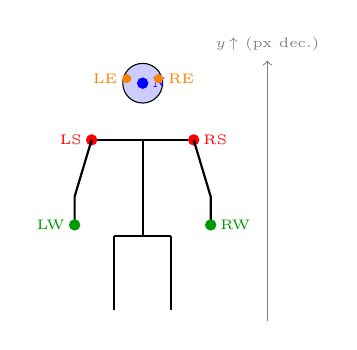
\begin{tikzpicture}[scale=0.72]
  \draw[fill=blue!20] (0,3.5) circle (0.35);
  \draw[thick] (-0.9,2.5) -- (0.9,2.5);
  \filldraw[red]           (-0.9,2.5) circle (0.09) node[left,  font=\tiny]{LS};
  \filldraw[red]           ( 0.9,2.5) circle (0.09) node[right, font=\tiny]{RS};
  \filldraw[blue]          (0,   3.5) circle (0.09) node[right, font=\tiny]{N};
  \filldraw[orange]        (-0.28,3.58) circle (0.07) node[left, font=\tiny]{LE};
  \filldraw[orange]        ( 0.28,3.58) circle (0.07) node[right,font=\tiny]{RE};
  \draw[thick] (-0.9,2.5) -- (-1.2,1.5) -- (-1.2,1.0);
  \draw[thick] ( 0.9,2.5) -- ( 1.2,1.5) -- ( 1.2,1.0);
  \filldraw[green!60!black](-1.2,1.0) circle (0.09) node[left,  font=\tiny]{LW};
  \filldraw[green!60!black]( 1.2,1.0) circle (0.09) node[right, font=\tiny]{RW};
  \draw[thick] (0,2.5) -- (0,0.8);
  \draw[thick] (-0.5,0.8) -- (0.5,0.8);
  \draw[thick] (-0.5,0.8) -- (-0.5,-0.5);
  \draw[thick] ( 0.5,0.8) -- ( 0.5,-0.5);
  \draw[->, gray, thin] (2.2,-0.7) -- (2.2,3.9)
        node[above, font=\tiny, gray]{$y\!\uparrow$ (px dec.)};
\end{tikzpicture}
\end{column}
\begin{column}{0.52\textwidth}
\footnotesize
\textbf{Key keypoints used:}
\begin{itemize}
    \item \textcolor{blue}{Nose} $(x_N, y_N)$
    \item \textcolor{orange}{Left/Right Ear} $(x_{LE},\,y_{LE})$
    \item \textcolor{red}{Left/Right Shoulder} $(x_{LS},\,y_{LS})$
    \item \textcolor{green!60!black}{Left/Right Wrist} $(x_{LW},\,y_{LW})$
\end{itemize}
\vspace{0.3cm}
\textbf{Note:} In image coords $y$ increases \emph{downward}, so wrist \emph{above} shoulder $\Rightarrow y_W < y_S$.
\end{column}
\end{columns}
\end{frame}

\begin{frame}{Math 1 --- Leaning Detection}
\textbf{Concept:} Measure how far the head deviates laterally from the shoulder midpoint.
\vspace{0.25cm}

\textbf{Step 1: Shoulder Centre}
\[ x_{SC} = \frac{x_{LS} + x_{RS}}{2} \]
\textbf{Step 2: Shoulder Width}
\[ W_S = |x_{LS} - x_{RS}| \]
\textbf{Step 3: Normalised Nose Offset Ratio}
\[ \boxed{R_{\text{lean}} = \frac{|x_N - x_{SC}|}{W_S}} \]
\textbf{Decision Rule:}
\[ \text{Leaning} = \begin{cases} \text{True} & R_{\text{lean}} > 0.4 \\ \text{False} & \text{otherwise} \end{cases} \]
\begin{alertblock}{Why normalise?}
Dividing by shoulder width makes the threshold \textbf{resolution-independent} --- works at 720p or 1080p without recalibration.
\end{alertblock}
\end{frame}

\begin{frame}{Math 2 --- Turning Back Detection}
\textbf{Concept:} As a student turns away, the visible ear-nose distances become asymmetric.
\vspace{0.2cm}
\[ d_L = \sqrt{(x_N-x_{LE})^2+(y_N-y_{LE})^2},\quad d_R = \sqrt{(x_N-x_{RE})^2+(y_N-y_{RE})^2} \]
\[ \boxed{R_{\text{turn}} = \frac{\min(d_L,\,d_R)}{\max(d_L,\,d_R)}} \]
\textbf{Decision Rule:}
\[ \text{Turning} = \begin{cases} \text{True} & R_{\text{turn}} < 0.15 \\ \text{False} & \text{otherwise} \end{cases} \]
\begin{columns}
\begin{column}{0.55\textwidth}
\footnotesize \textbf{Geometric Intuition:}
\begin{itemize}
    \item Face-forward: $d_L \approx d_R \Rightarrow R \approx 1.0$
    \item $60^\circ$ rotation: far ear occludes $\Rightarrow R \approx 0.15$
    \item Fully turned: $R \approx 0.0$
\end{itemize}
\end{column}
\begin{column}{0.45\textwidth}
\begin{block}{Why 0.15?}
Captures rotations $>60^\circ$ --- the minimum angle to view a neighbour's paper.
\end{block}
\end{column}
\end{columns}
\end{frame}

\begin{frame}{Math 3 --- Hand Raise Detection}
\textbf{Concept:} In image coordinates ($y=0$ at top), a raised wrist has a \emph{smaller} $y$-value than the shoulder.
\vspace{0.3cm}

\textbf{Vertical Offset:}
\[ y_{S,\min} = \min(y_{LS},\;y_{RS}) \]
\[ \boxed{\delta_W = y_{S,\min} - y_W \quad \text{(positive when wrist is above shoulder)}} \]
\textbf{Decision Rule:}
\[ \text{HandRaised} = \begin{cases} \text{True} & \delta_W > 20\;\text{px} \\ \text{False} & \text{otherwise} \end{cases} \]
\begin{block}{Why 20 px margin + 5 frames?}
\begin{itemize}
    \item The 20 px margin eliminates accidental triggers (adjusting glasses, scratching).
    \item 5 consecutive frames (vs.\ 3 for others) because brief arm lifts are very common.
\end{itemize}
\end{block}
\end{frame}

\begin{frame}{Math 4 --- Passing Paper Detection}
\textbf{Concept:} Flag when two students' wrists converge within a dual-threshold proximity box.
\vspace{0.15cm}

For students $A$ and $B$:
\[ \Delta x = |x_{W_A} - x_{W_B}|, \qquad \Delta y = |y_{W_A} - y_{W_B}| \]
\[ \boxed{ \text{PassingPaper} = \begin{cases} \text{True} & \Delta x < 200\;\text{px} \;\textbf{AND}\; \Delta y < 150\;\text{px} \\ \text{False} & \text{otherwise} \end{cases} } \]
\begin{columns}
\begin{column}{0.55\textwidth}
\footnotesize \textbf{Why dual thresholds (not Euclidean)?}
\begin{itemize}
    \item Euclidean fails for students in different rows.
    \item Horizontal (200 px): catches same-row convergence.
    \item Vertical (150 px): excludes different rows.
\end{itemize}
\end{column}
\begin{column}{0.45\textwidth}
\centering
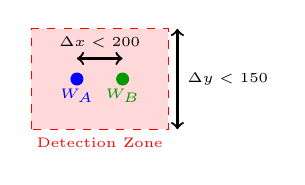
\begin{tikzpicture}[scale=0.58]
  \draw[fill=red!15,draw=red,dashed](-1.5,-1.1) rectangle (1.5,1.1);
  \filldraw[blue]          (-0.5,0) circle (0.13) node[below,font=\tiny]{$W_A$};
  \filldraw[green!60!black]( 0.5,0) circle (0.13) node[below,font=\tiny]{$W_B$};
  \draw[<->,thick](-0.5,0.45)--(0.5,0.45) node[midway,above,font=\tiny]{$\Delta x<200$};
  \draw[<->,thick](1.7,-1.1)--(1.7,1.1)   node[midway,right,font=\tiny]{$\Delta y<150$};
  \node[font=\tiny,red] at (0,-1.4){Detection Zone};
\end{tikzpicture}
\end{column}
\end{columns}
\end{frame}

\begin{frame}{Math 5 --- Mobile Phone Detection}
\textbf{Concept:} YOLO classifies object as COCO class 67. Smart filters eliminate false positives.
\vspace{0.2cm}

\textbf{Detection Condition:}
\[ \text{PhoneDetected} = \begin{cases} \text{True} & c_{67} \geq 0.25 \;\wedge\; \text{IsNearHand}(\text{bbox}) \\ \text{False} & \text{otherwise} \end{cases} \]
\textbf{Oversized Bounding Box Filter:}
\[ \text{Reject if}\quad \frac{w_{\text{bbox}}\times h_{\text{bbox}}}{W\times H} > 0.15 \;\wedge\; c_{67} < 0.4 \]
\textbf{Aspect Ratio Filter:}
\[ \text{Reject if}\quad \left|\frac{w_{\text{bbox}}}{h_{\text{bbox}}} - 1\right| < 0.2 \;\wedge\; c_{67} < 0.4 \]
\begin{alertblock}{Result}
Threshold $\tau = 0.25$ achieves $\sim$92\% TPR with $<$14\% FPR in classroom conditions.
\end{alertblock}
\end{frame}

\begin{frame}{Math 6 --- Consecutive Frame Thresholding}
\textbf{Problem:} Single-frame detection triggers $\approx$70\% false positives.

\textbf{Solution:} A temporal counter $C_t$ per detection type:
\[ C_t = \begin{cases} C_{t-1} + 1 & \text{malpractice detected in frame }t \\ \max(0,\;C_{t-1}-1) & \text{otherwise} \end{cases} \]
\[ \boxed{\text{Flag Incident} \iff C_t \geq \Theta_{\text{type}}} \]
\begin{center}
\footnotesize
\begin{tabular}{lcc}
\toprule
\textbf{Type} & $\Theta_{\text{type}}$ & \textbf{Grace Period (frames)} \\
\midrule
Mobile Phone  & 5 & 60 \\
Hand Raised   & 5 & 60 \\
Leaning       & 3 & 60 \\
Turning Back  & 3 & 60 \\
Passing Paper & 3 & 60 \\
\bottomrule
\end{tabular}
\end{center}
\begin{block}{Grace Period}
After detection ends, records 60 more frames ($\approx$2 s) to capture the complete incident.
\end{block}
\end{frame}

\begin{frame}{Math 7 --- AI Probability Scoring (Live Stream)}
\textbf{Formula 1: Live Camera Streams}
\[ P_{\text{base}} = \frac{N_{\text{detect}}}{N_{\text{total}}} \times 100 \]
\begin{itemize}
    \item $N_{\text{detect}}$ = frames in which malpractice was detected
    \item $N_{\text{total}}$ = total ML-processed frames
\end{itemize}
A \textbf{confidence bonus} is added:
\[ \boxed{P_{\text{live}} = P_{\text{base}} + \alpha \cdot \bar{c}_{\text{YOLO}}} \]
\begin{exampleblock}{Example}
Mobile phone detected in 45/60 frames, mean YOLO conf 0.78:\\
$P_{\text{base}} = \dfrac{45}{60} \times 100 = 75\%,\quad P_{\text{final}} \approx 83\%$
\end{exampleblock}
\end{frame}

\begin{frame}{Math 7 --- AI Probability Scoring (Uploaded Videos)}
\textbf{Formula 2: Uploaded / Legacy Videos}
\[ \boxed{P_{\text{upload}} = \bigl(0.60\times S_{\text{dur}} + 0.40\times S_{\text{prior}}\bigr)\times 100} \]
\begin{columns}
\begin{column}{0.5\textwidth}
\footnotesize \textbf{Duration Score $S_{\text{dur}}$:}
\begin{tabular}{ll}
\toprule
Clip Length & Score \\ \midrule
$\geq10$ s & 1.00 \\ $\geq6$ s & 0.90 \\ $\geq4$ s & 0.75 \\ $\geq2$ s & 0.55 \\ $\geq1$ s & 0.30 \\ $<1$ s & 0.20 \\
\bottomrule
\end{tabular}
\end{column}
\begin{column}{0.5\textwidth}
\footnotesize \textbf{Type Prior $S_{\text{prior}}$:}
\begin{tabular}{ll}
\toprule
Behavior & Prior \\ \midrule
Mobile Phone & 0.80 \\ Turning Back & 0.70 \\ Leaning & 0.60 \\ Passing Paper & 0.55 \\ Hand Raise & 0.45 \\
\bottomrule
\end{tabular}
\end{column}
\end{columns}
\vspace{0.3cm}
\begin{exampleblock}{Example}
Mobile phone clip of 7 s: $P = (0.60\times0.90 + 0.40\times0.80)\times100 = \mathbf{86\%}$
\end{exampleblock}
\end{frame}

\begin{frame}{Math 8 --- Evaluation Metrics}
TP = True Positive \quad TN = True Negative \quad FP = False Positive \quad FN = False Negative
\vspace{0.3cm}
\begin{columns}
\begin{column}{0.5\textwidth}
\[ \text{Accuracy} = \frac{TP+TN}{TP+TN+FP+FN} \]
\[ \text{Precision} = \frac{TP}{TP+FP} \]
\end{column}
\begin{column}{0.5\textwidth}
\[ \text{Recall} = \frac{TP}{TP+FN} \]
\[ F_1 = 2\cdot\frac{\text{Precision}\times\text{Recall}}{\text{Precision}+\text{Recall}} \]
\end{column}
\end{columns}
\vspace{0.4cm}
\begin{block}{Interpretation for AIInvigilator}
\begin{itemize}
    \item \textbf{High Precision} $\Rightarrow$ few false alarms (invigilator trust)
    \item \textbf{High Recall} $\Rightarrow$ few missed incidents (exam integrity)
    \item \textbf{F1} balances both --- our primary optimisation target
\end{itemize}
\end{block}
\end{frame}

\begin{frame}{Mathematical Summary}
\begin{center}
\footnotesize
\renewcommand{\arraystretch}{1.4}
\begin{tabular}{lll}
\toprule
\textbf{Detection} & \textbf{Core Formula} & \textbf{Threshold} \\
\midrule
Leaning       & $R_{\text{lean}} = \dfrac{|x_N - x_{SC}|}{W_S}$ & $> 0.4$ \\[6pt]
Turning Back  & $R_{\text{turn}} = \dfrac{\min(d_L,d_R)}{\max(d_L,d_R)}$ & $< 0.15$ \\[6pt]
Hand Raise    & $\delta_W = y_{S,\min} - y_W$ & $> 20$\,px \\[4pt]
Passing Paper & $\Delta x < 200\,\text{px} \wedge \Delta y < 150\,\text{px}$ & Dual \\[4pt]
Mobile Phone  & YOLO conf $c_{67}$ & $\geq 0.25$ \\
\midrule
\multicolumn{2}{l}{\textbf{AI Score (Live):}} & $\frac{N_d}{N_t}\times100 + \text{bonus}$ \\[4pt]
\multicolumn{2}{l}{\textbf{AI Score (Upload):}} & $(0.6\,S_{\text{dur}}+0.4\,S_{\text{prior}})\times100$ \\
\bottomrule
\end{tabular}
\end{center}
\vspace{0.3cm}
\begin{block}{Key Design Principle}
All thresholds are \textbf{normalised} (resolution-independent) or \textbf{empirically calibrated} on 200--300+ real classroom frames to minimise FP while maximising detection rate.
\end{block}
\end{frame}

% ================================================================
%  SYSTEM DEMO DIVIDER
% ================================================================
\begin{frame}{}
    \centering
    \Huge \textbf{System Working Demonstration}
\end{frame}

% ================================================================
\section{System Working Demonstration}
% ================================================================
\begin{frame}{Home Page}
\centering
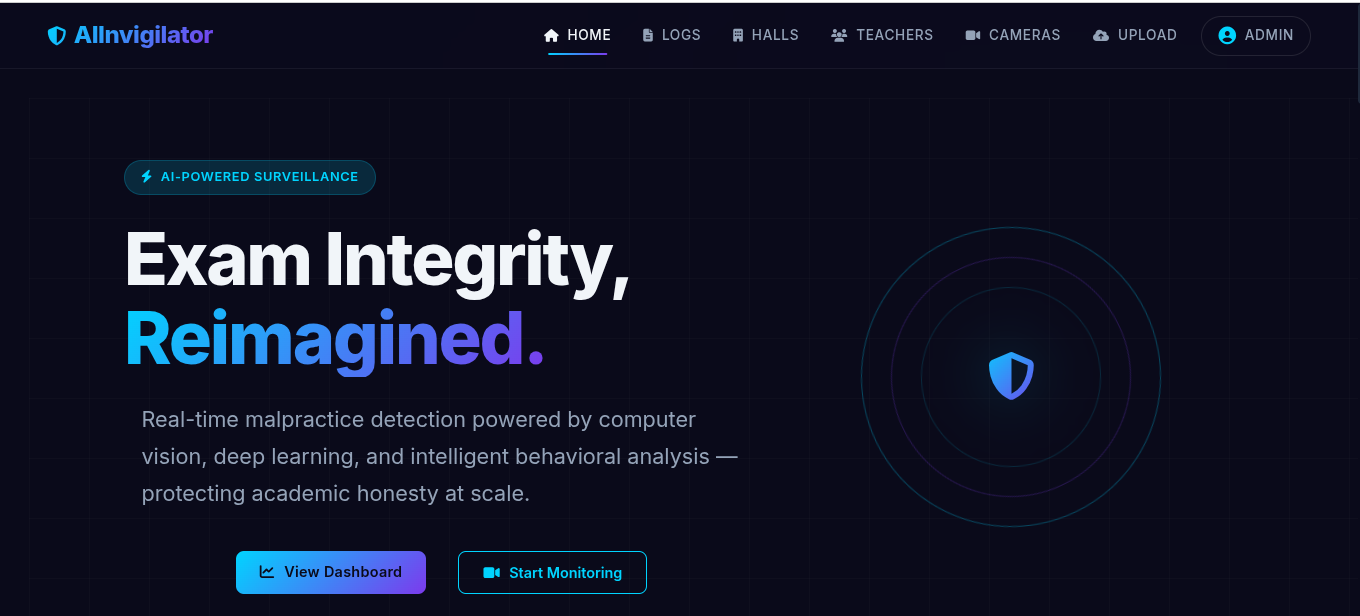
\includegraphics[width=0.9\linewidth]{home_page.png}
\vspace{0.3cm}
\small Home page of AI Invigilator system showing navigation options.
\end{frame}

\begin{frame}{Login Page}
\centering
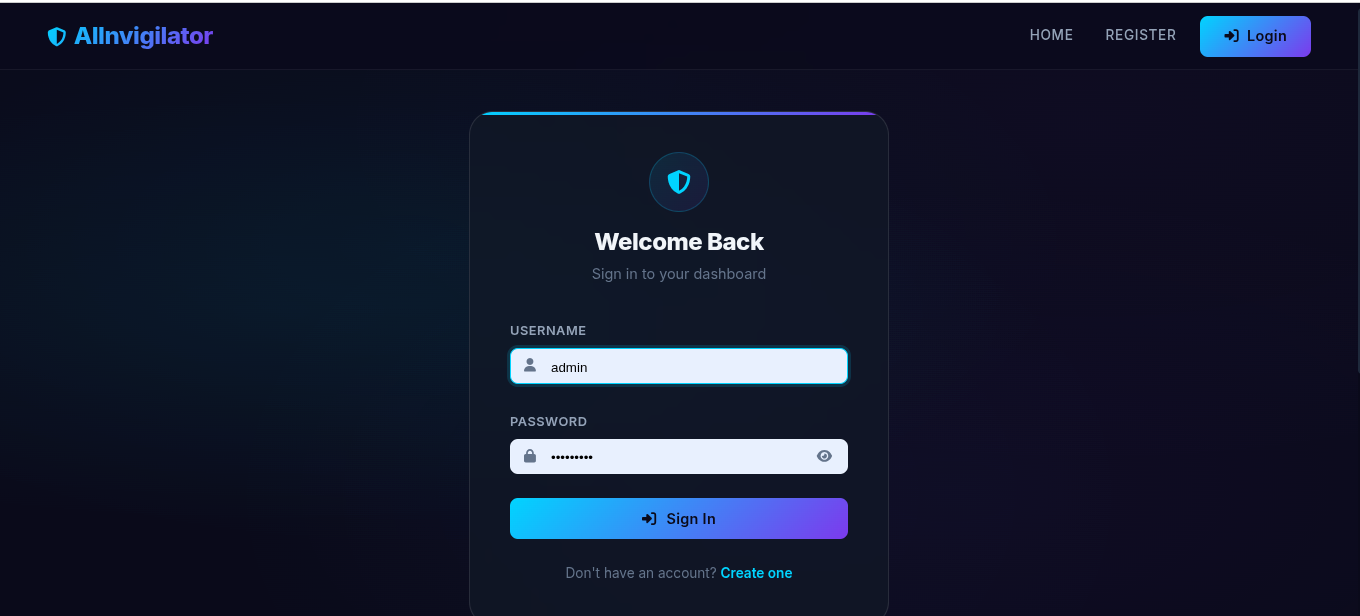
\includegraphics[width=0.9\linewidth]{login_page.png}
\vspace{0.3cm}
\small Secure login for administrators and faculty members.
\end{frame}

\begin{frame}{Teacher Registration}
\centering
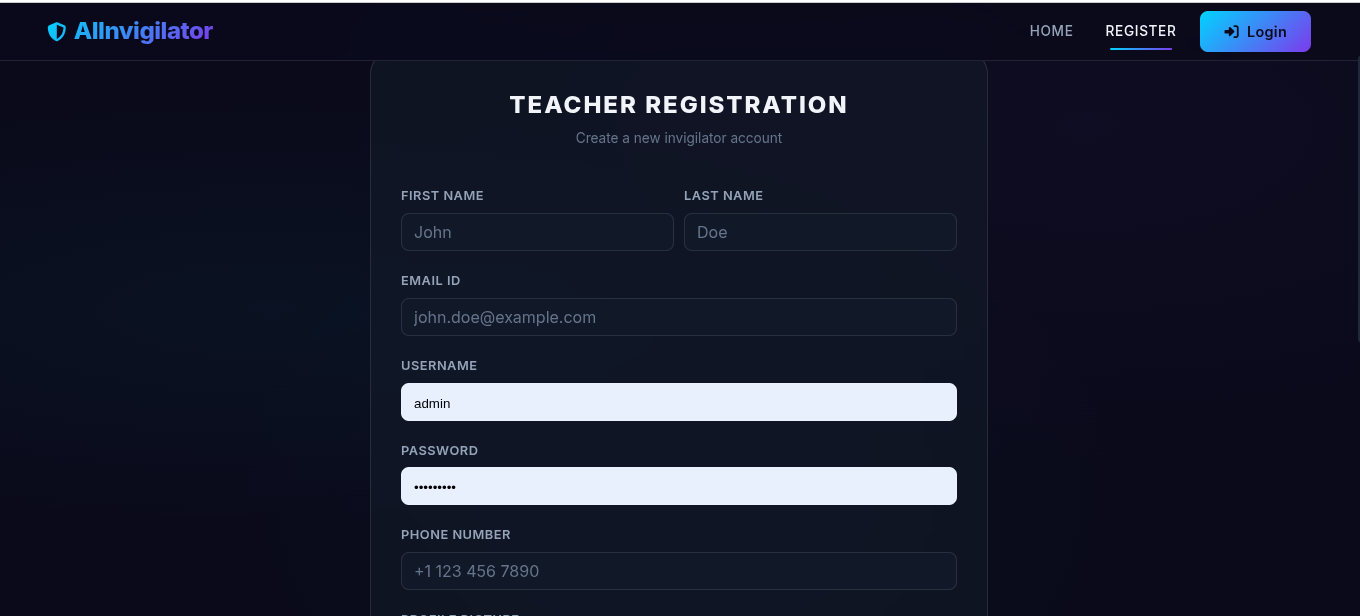
\includegraphics[width=0.9\linewidth]{teacher_registration.png}
\vspace{0.3cm}
\small New teachers can register here.
\end{frame}

\begin{frame}{Exam Hall Management}
\centering
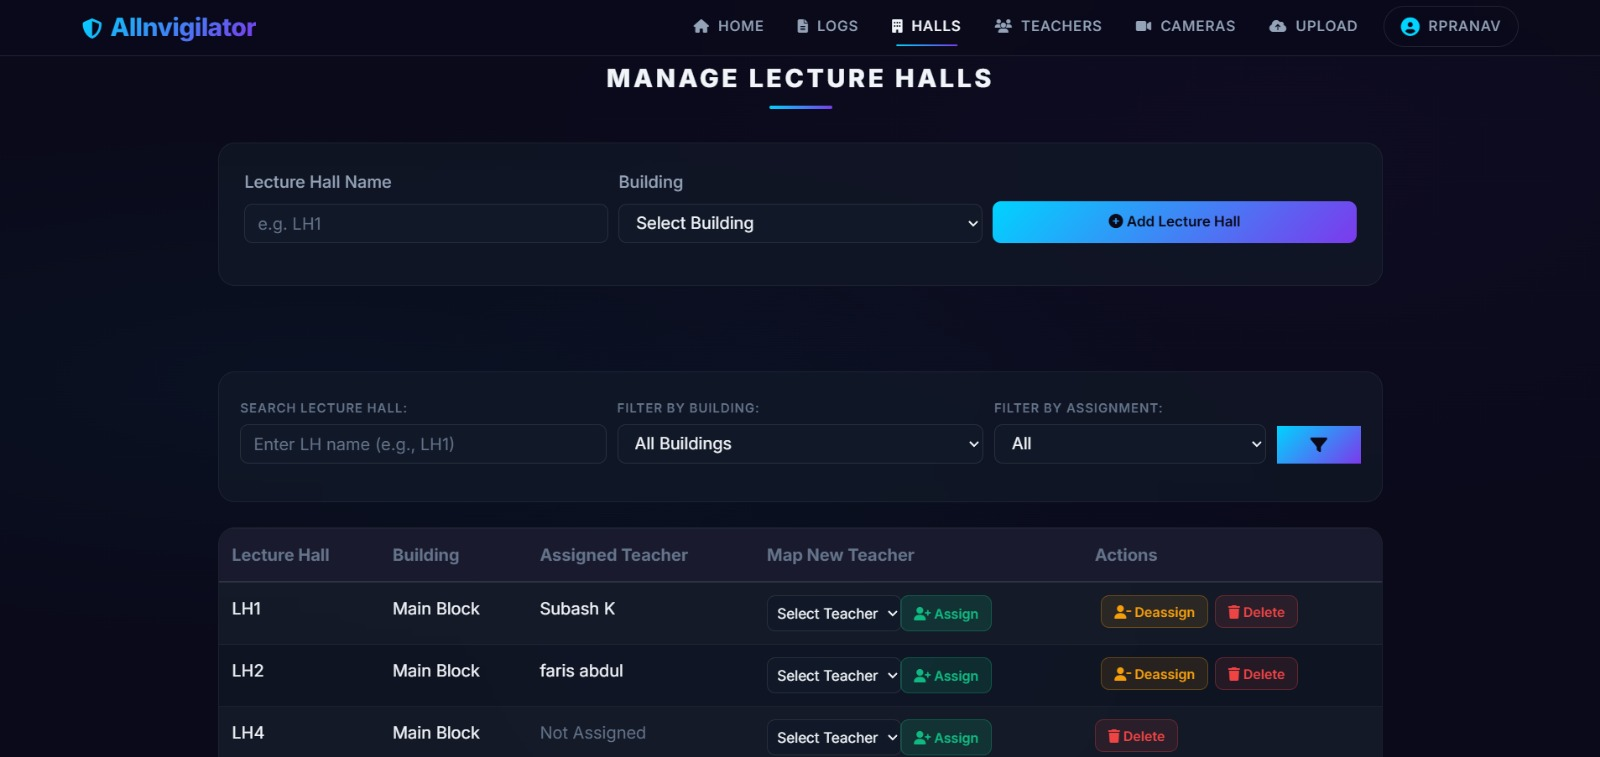
\includegraphics[width=0.9\linewidth]{exam_hall.jpeg}
\vspace{0.3cm}
\small Interface to manage and configure lecture halls.
\end{frame}

\begin{frame}{Teacher Logs}
\centering
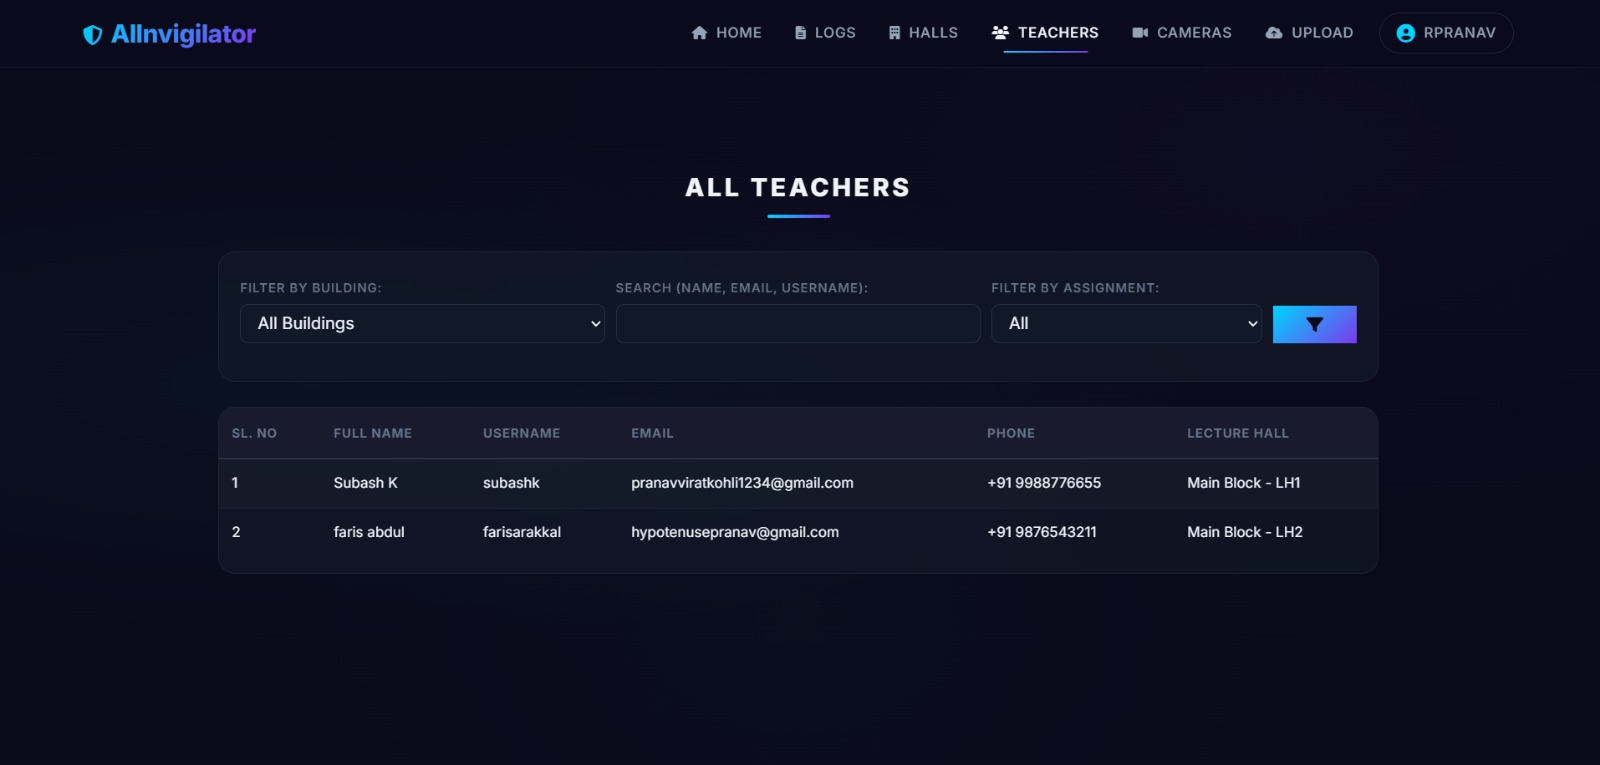
\includegraphics[width=0.9\linewidth]{teachers.jpeg}
\vspace{0.3cm}
\small Here we can see all the teachers that are logged in.
\end{frame}

\begin{frame}{Front View Detection -- Turning Back}
\centering
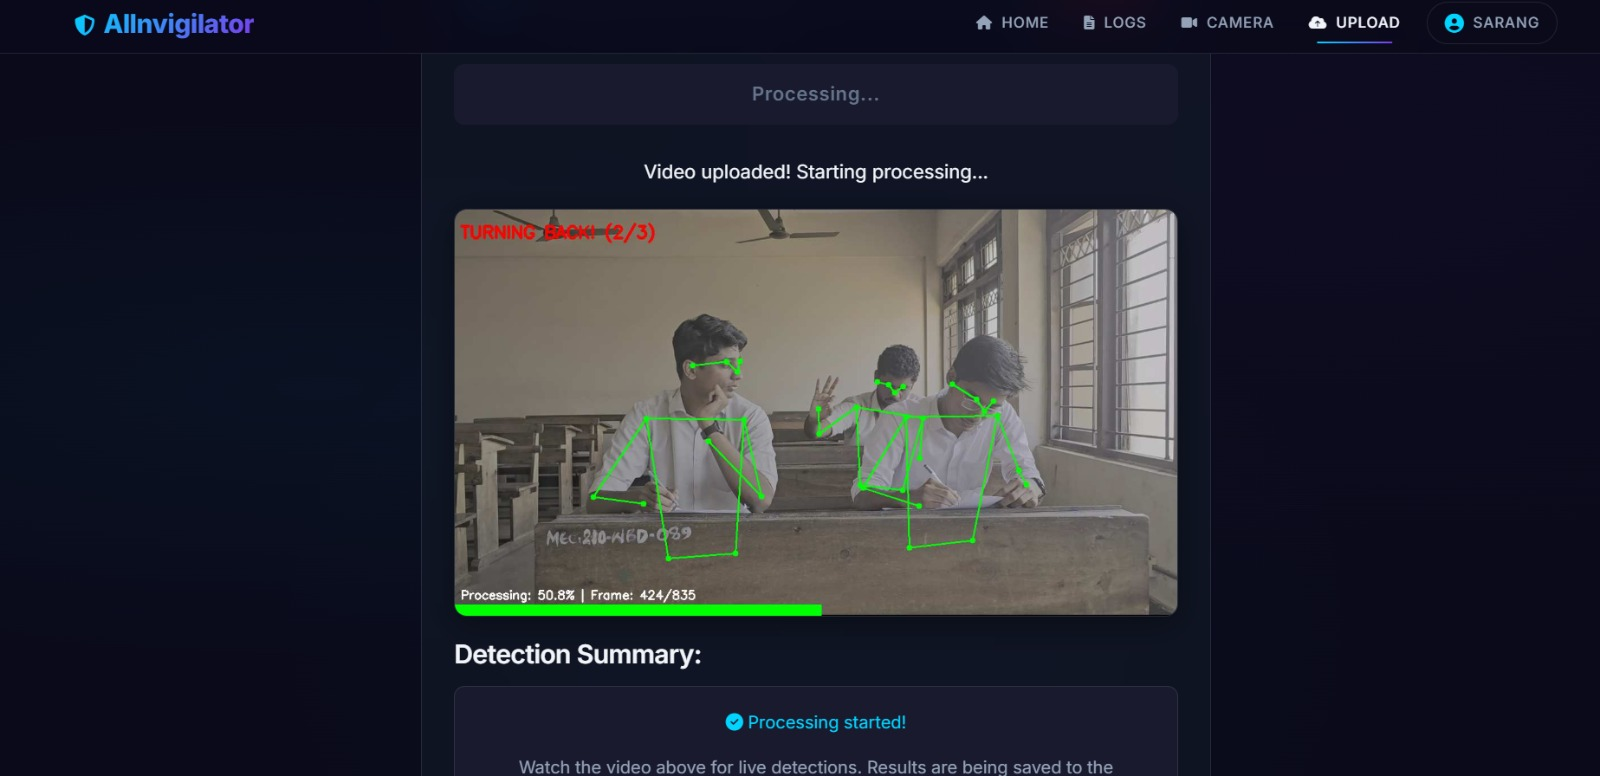
\includegraphics[width=0.9\linewidth]{front_view1.jpeg}
\vspace{0.3cm}
\small Real-time pose-based detection of suspicious posture (turning back).
\end{frame}

\begin{frame}{Front View Detection -- Passing Paper}
\centering
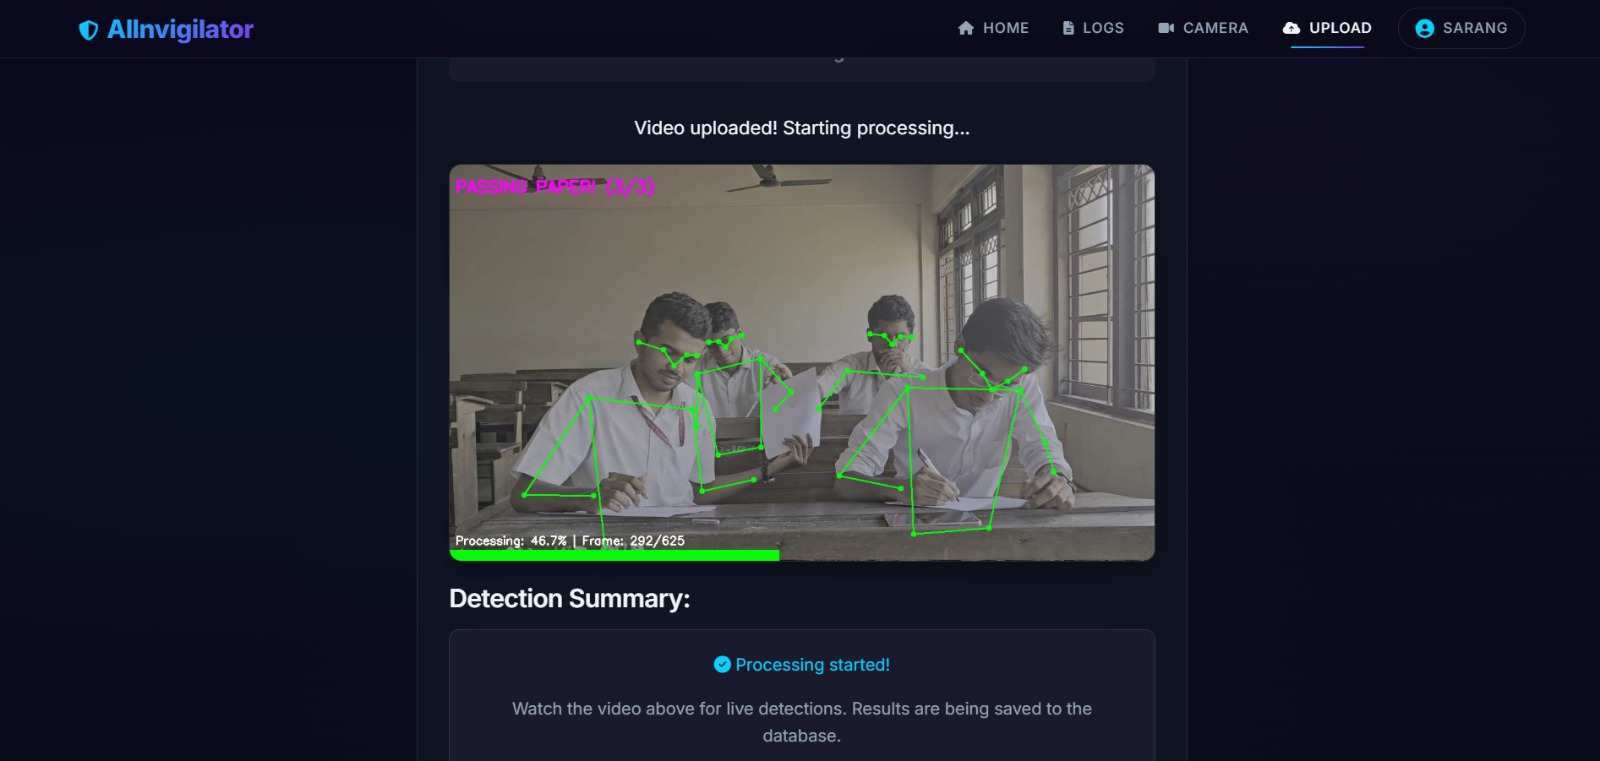
\includegraphics[width=0.9\linewidth]{front_view2.jpeg}
\vspace{0.3cm}
\small Real-time pose-based detection of suspicious posture (passing paper).
\end{frame}

\begin{frame}{Top View Detection -- Passing Paper}
\centering
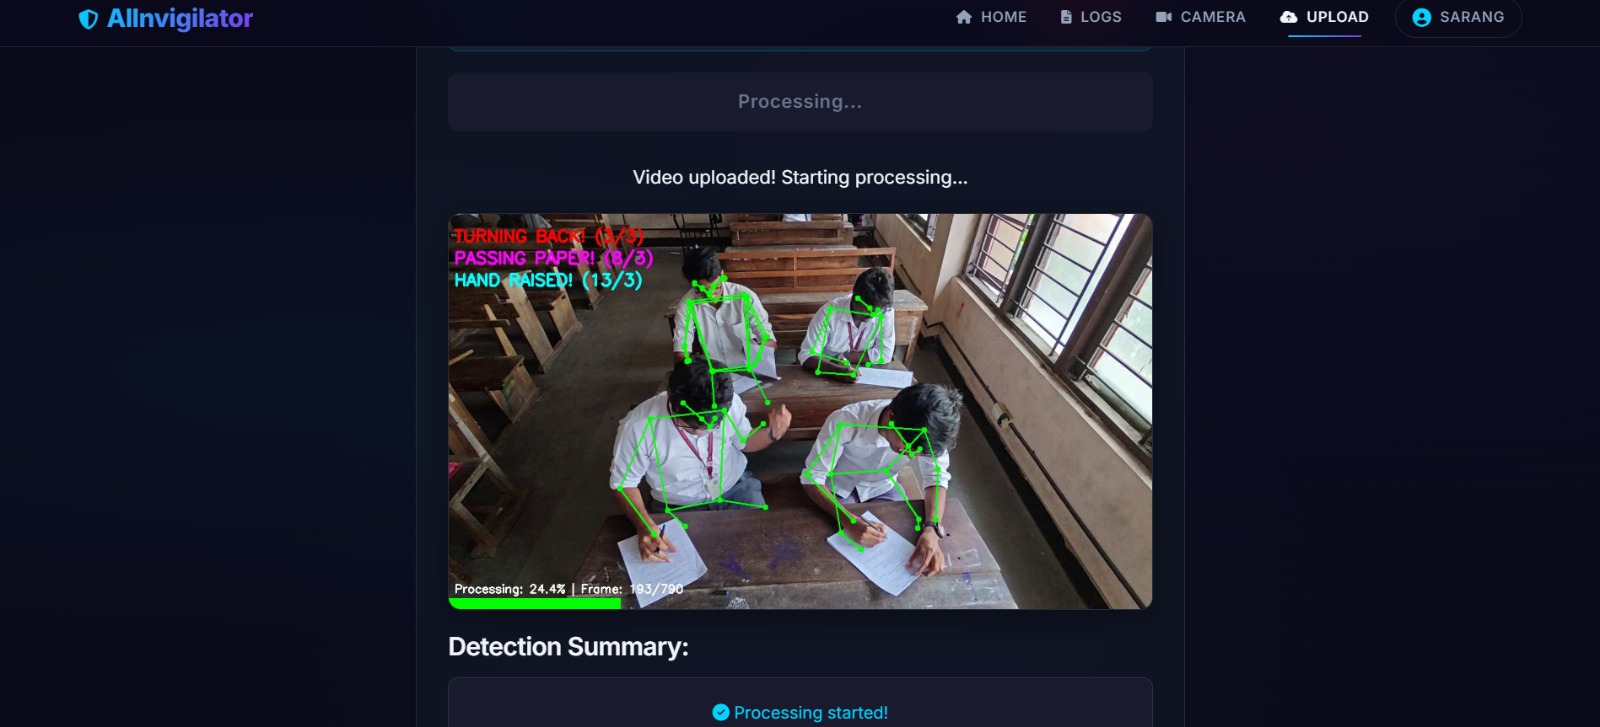
\includegraphics[width=0.9\linewidth]{top_view1.jpeg}
\vspace{0.3cm}
\small Detection of malpractice (passing paper) from Top view.
\end{frame}

\begin{frame}{Top View Detection -- Leaning}
\centering
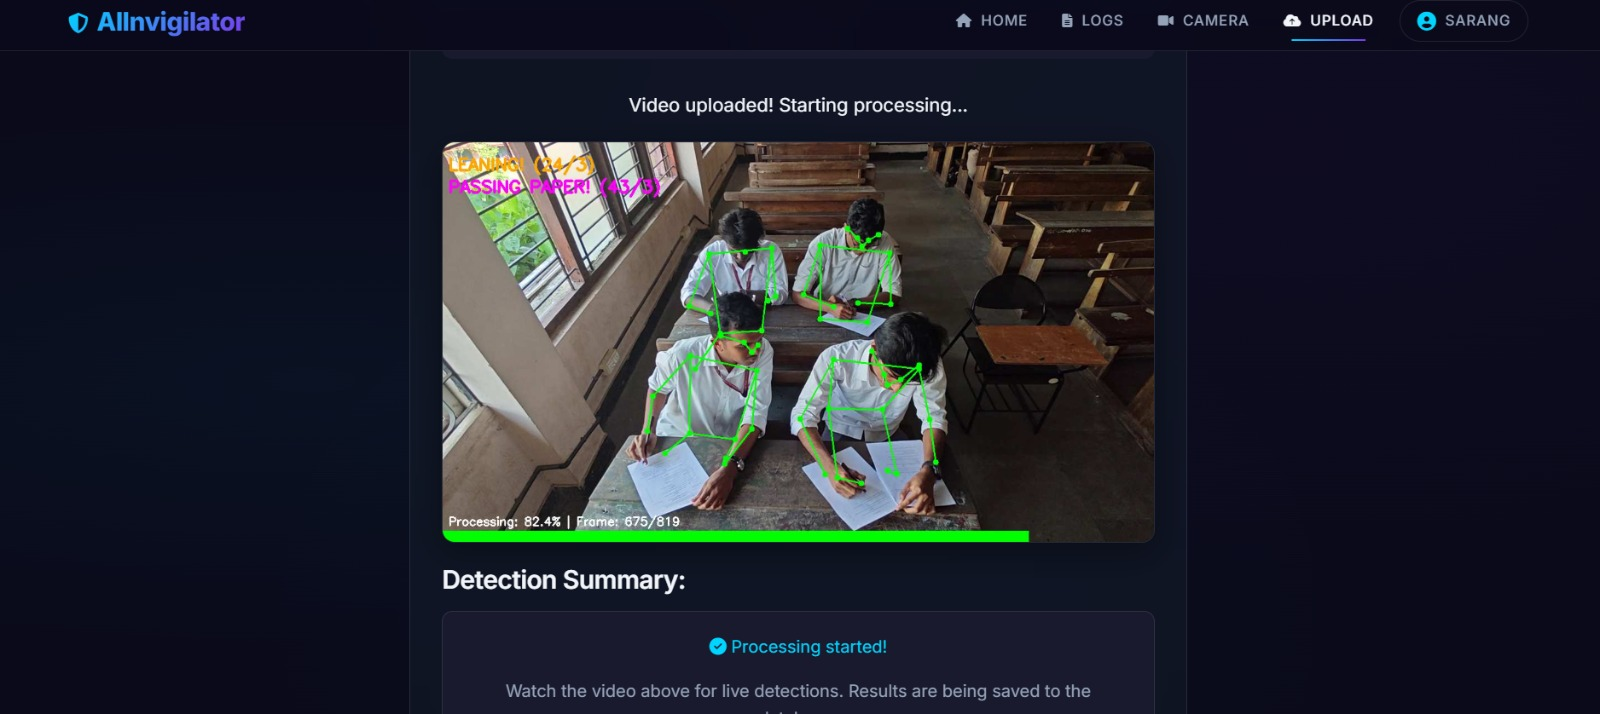
\includegraphics[width=0.9\linewidth]{top_view2.jpeg}
\vspace{0.3cm}
\small Detection of malpractice (leaning) from Top view.
\end{frame}

\begin{frame}{Malpractice Logs}
\centering
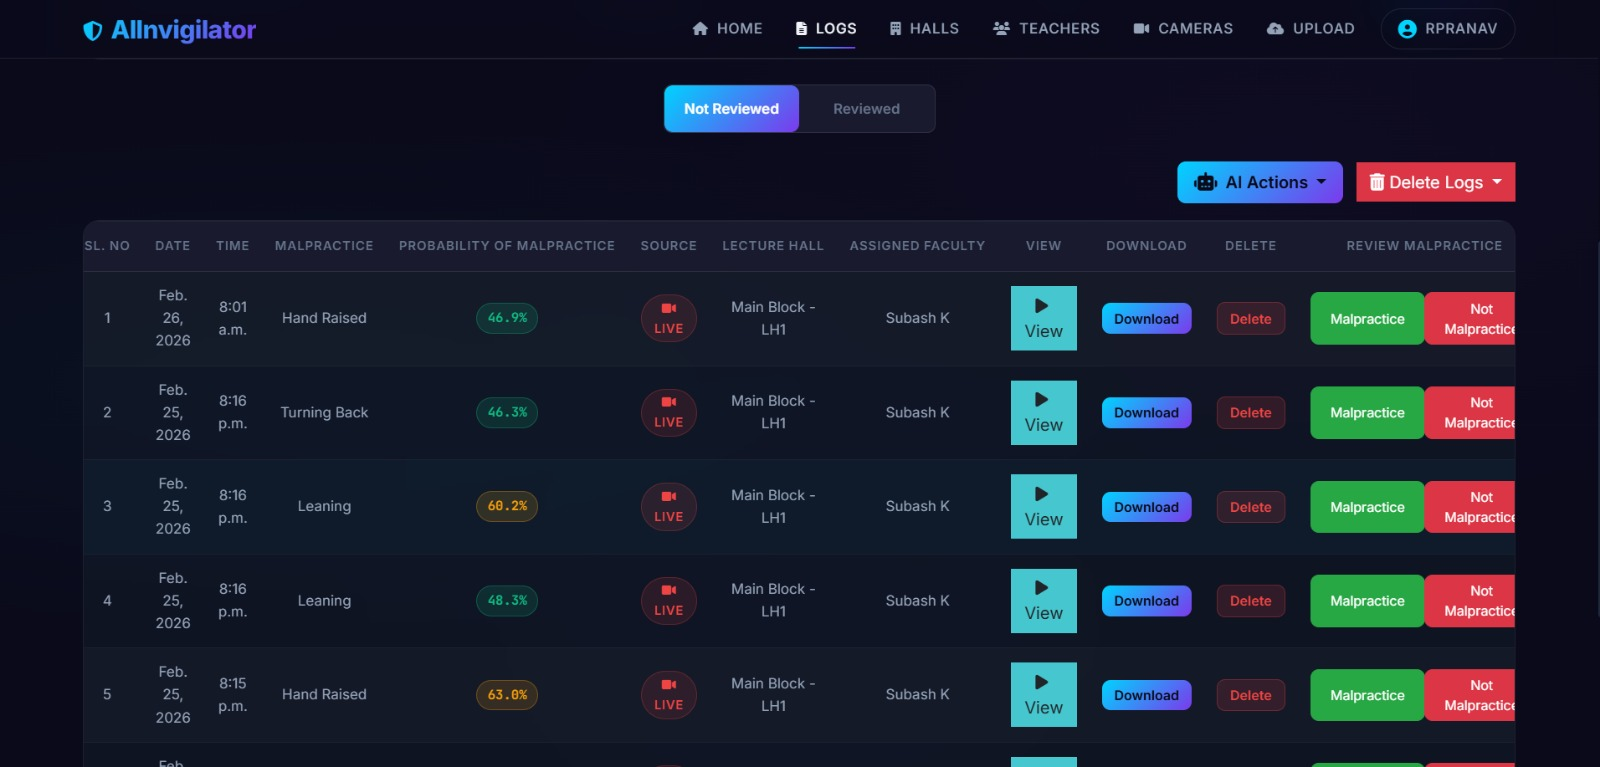
\includegraphics[width=0.9\linewidth]{logs.jpeg}
\vspace{0.3cm}
\small Database records of detected incidents with timestamps.
\end{frame}

\begin{frame}{Email Alert Notification}
\centering
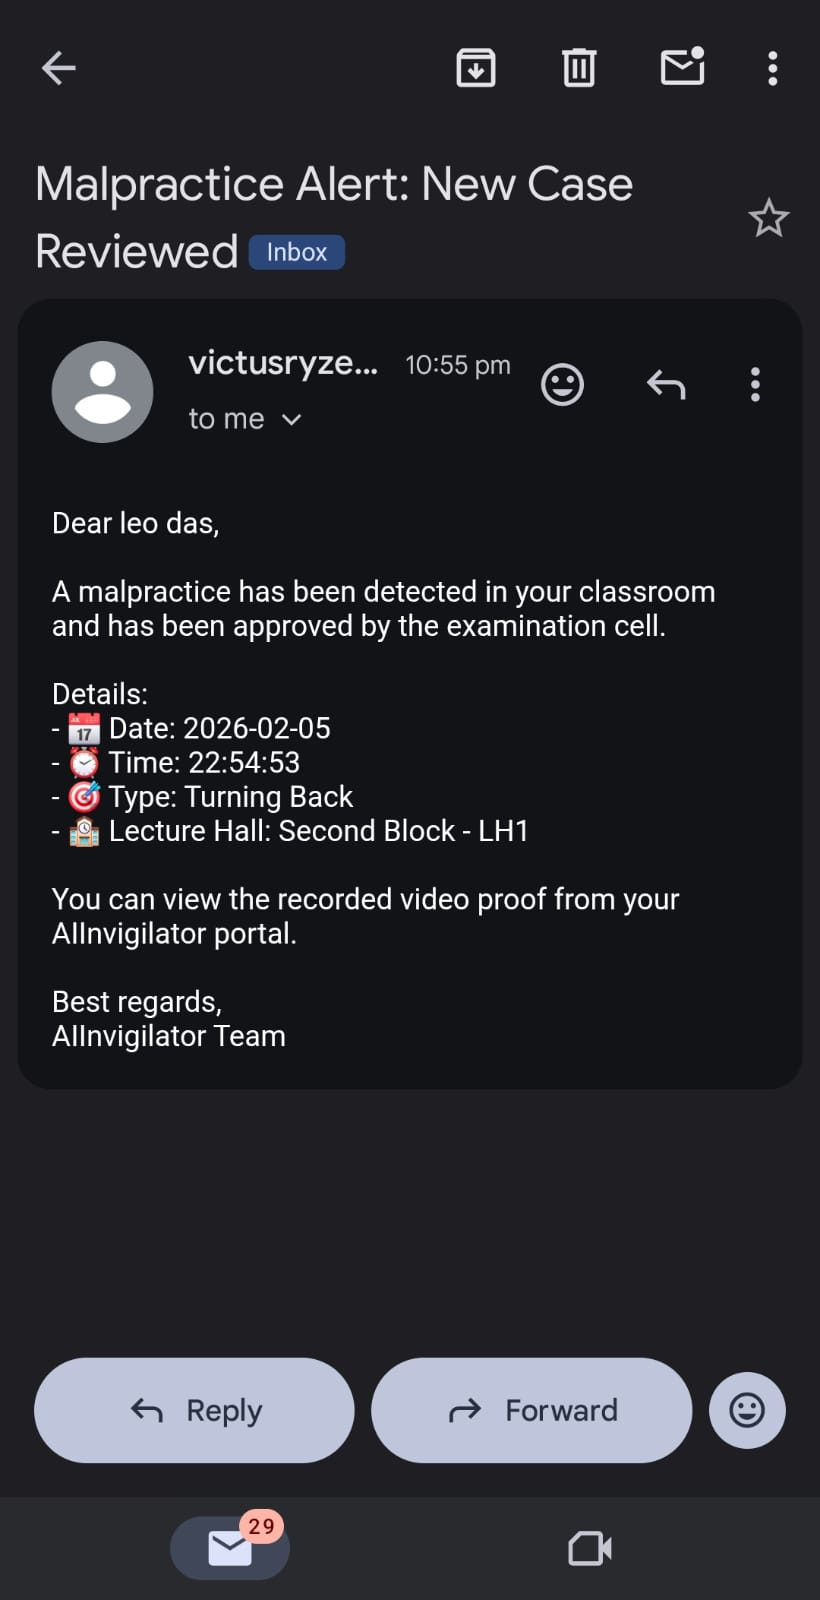
\includegraphics[height=0.75\textheight, keepaspectratio]{Alert.jpeg}
\vspace{0.3cm}
\small Automated email alert sent to proctor when malpractice is detected.
\end{frame}

% ================================================================
\section{Evaluation Metrics \& Performance}
% ================================================================
\begin{frame}{Evaluation Metrics}
Standard evaluation metrics used to assess system performance:
\begin{table}[]
\centering
\resizebox{0.9\textwidth}{!}{
\begin{tabular}{|l|c|c|c|c|}
\hline
\textbf{Detection Type} & \textbf{Precision} & \textbf{Recall} & \textbf{F1 Score} & \textbf{Accuracy} \\ \hline
Mobile Phone  & 0.90 & 0.85 & 0.87 & 0.88 \\ \hline
Hand Raised   & 0.88 & 0.90 & 0.89 & 0.91 \\ \hline
Turning Back  & 0.85 & 0.80 & 0.82 & 0.86 \\ \hline
Leaning       & 0.82 & 0.78 & 0.80 & 0.84 \\ \hline
Passing Paper & 0.78 & 0.72 & 0.75 & 0.80 \\ \hline
\end{tabular}
}
\end{table}
\vspace{0.3cm}
\tiny Source: Detection Performance Metrics by Malpractice Type
\end{frame}

\begin{frame}{Performance Results}
\begin{itemize}
    \item \textbf{Inference Speed:} YOLOv11n achieves $\sim65$ FPS and YOLO-Pose achieves $\sim45$ FPS on an NVIDIA RTX 3050. Combined pipeline processes at $\geq15$ FPS per stream.
    \item \textbf{Alert Latency:} Average time from detection to dashboard notification is $<1.5$ seconds.
    \item \textbf{False Positive Reduction:} Consecutive frame thresholding reduces false positives by approximately $70\%$ compared to single-frame detection.
\end{itemize}
\end{frame}

% ================================================================
\section{Project Evaluation \& Impact}
% ================================================================
\begin{frame}{Project Evaluation \& Impact}
\footnotesize
\begin{itemize}
    \item Addressed the lack of intelligent real-time monitoring in examination halls
    \item Collected and labeled a custom classroom dataset for malpractice detection
    \item Trained a YOLO-based model for object detection and behavioral recognition
    \item Integrated geometry-based validation rules for reliable gesture analysis
    \item Built a complete real-time alerting and logging pipeline
    \item System functions successfully; FPS currently limited by hardware constraints
    \item Scalable to multiple classrooms with performance optimization
\end{itemize}
\end{frame}

% ================================================================
\section{Future Scope}
% ================================================================
\begin{frame}{Future Scope}
\begin{itemize}
    \item \textbf{LSTM-Based Temporal Analysis:} Integrate Long Short-Term Memory networks for analyzing sequences of poses over time to detect gradually unfolding behaviors.
    \item \textbf{Multi-Camera Fusion:} Correlate detections across multiple cameras in the same hall for enhanced spatial understanding and reduced blind spots.
    \item \textbf{Audio-Based Analysis:} Incorporate speech detection models to identify whispering or verbal communication.
    \item \textbf{Vision-Language Models (VLMs):} Leverage VLMs for context-aware interpretation of detected events to further reduce false positives.
\end{itemize}
\end{frame}

% ================================================================
\section{Conclusion}
% ================================================================
\begin{frame}{Conclusion}
\begin{itemize}
    \item The \textbf{AIInvigilator} project addresses the critical need for intelligent, automated monitoring to overcome the limitations of traditional manual proctoring in exam environments.
    \item By combining real-time object detection and pose estimation, the system accurately identifies potential malpractice, providing a crucial layer of security and oversight.
    \item The primary goal is to provide a scalable and low-resource tool that empowers human invigilators, enhances fairness, and upholds the integrity of the entire examination process.
    \item Ultimately, AIInvigilator contributes to the broader effort of modernizing educational technology, ensuring academic standards are maintained in an efficient, reliable, and fair manner.
\end{itemize}
\end{frame}

% ================================================================
%  THANK YOU
% ================================================================
\begin{frame}{}
    \centering
    \Huge Thank You!
\end{frame}

\end{document}